\section*{Component specific Types}

\begin{table}[!htb] 
    \label{api:selectComponentTypes}
    \footnotesize
    \setlength\extrarowheight{4pt}
    \begin{tabular}{ p{5cm} p{8cm}}
        \toprule[1.2pt]
        \textbf{Type}    & \textbf{Description} \\
        \midrule    
        SimpleOptionType & \{ label: String?, value: String \}    \\
        OptionDataType   & \{ String | SimpleOptionType \}        \\
        OptionsTable     & Array$<$Array$<$OptionDataType$>>$       \\
        CallbackType     & (...String) => Array$<$OptionDataType$>$ \\
        \bottomrule[1.2pt]
    \end{tabular}
\end{table}

\vspace*{12pt}
The \codestyle{SelectAttributes} object contains the following properties: 

\begin{table}[!htb] 
    \label{api:selectComponentSelectAttributes}
    \footnotesize
    \setlength\extrarowheight{4pt}
    \begin{tabular}{ p{4cm} p{3cm} p{6cm} }
        \toprule[1.2pt]
        \textbf{Property}             & \textbf{Type} & \textbf{Description} \\
        \midrule
        label                         & String        & Content of the Label for the input. \\
        name                          & String        & Name of the input that is sent with the form. \\
        isRequired                    & Boolean       & Defines if the selection of an option is required to send the form. \\
        isDisabled                    & Boolean       & Defines if the value can be changedand if the interaction work. \\
        isCursorPositionWithSelection & Boolean       & Defines if the cursor position is linked with the selection. 
                                                        If true: the keyboard interaction directly changes the selection. \\
        \bottomrule[1.2pt]
    \end{tabular}
\end{table}


% ---------
\clearpage
\section*{Components}

\vspace*{6pt}
\subsection*{SelectComponentByCallbacks}

\vspace*{6pt}
Creates an input component with the functionality: selecting an option in a given list. 

\vspace*{18pt}
\noindent
\textbf{Returns}: \codestyle{SelectComponentType}

\begin{table}[!htb] 
    \label{api:selectComponentByCallbacksReturn}
    \footnotesize
    \setlength\extrarowheight{4pt}
    \begin{tabular}{ p{3.5cm} p{3.5cm} p{6cm} }
        \toprule[1.2pt]
        \textbf{Function}     & \textbf{Type}        & \textbf{Description} \\
        \midrule
        getSelectController() & SelectControllerType &  \\
        getComponentView()    & HTMLDivElement       &  \\
        getLabelElement()     & HTMLLabelElemen      &  \\
        \bottomrule[1.2pt]
    \end{tabular}
\end{table}

\vspace*{6pt}
\noindent
\textbf{Parameters}

\begin{table}[!htb] 
    \label{api:selectComponentByCallbacksParameter}
    \footnotesize
    \setlength\extrarowheight{4pt}
    \begin{tabular}{ p{3.5cm} p{3.5cm} p{6cm} }
        \toprule[1.2pt]
        \textbf{Name}    & \textbf{Type}       & \textbf{Description} \\
        \midrule
        selectAttributes & SelectAttributes    &  \\
        serviceCallbacks & Array<CallbackType> &  \\
        \bottomrule[1.2pt]
    \end{tabular}
\end{table}

\vspace*{6pt}
\noindent
\textbf{Example}

\begin{lstlisting}[style = htmlcssjs, label = api:selectComponentCbExample]
const getYearsByDecade = (...decades) => {
    const decadeStarts = decades.map(decade => decade.slice(0, 3));
    const data         = [...Array(70).keys()].map((e) => e + 1940 + "");
    return data.filter((e) => decadeStarts.length === 0 || decadeStarts.includes(e.slice(0, 3)));
};
const getDecades = () => [...Array(7).keys()].map((e) => e * 10 + 1940 + "'s");

const selectAttribute = { name : "year", label: "Year" };
const columnServiceCb = [ getDecades, getYearsByDecade ];

const selectComponent = SelectComponentByCallbacks(
    selectAttribute,
    columnServiceCb
);

const componentYear   = document.getElementById("componentContainer");
componentYear.append(selectComponent.getComponentView());
\end{lstlisting}
    
\begin{figure}[!htb]
    \centering
    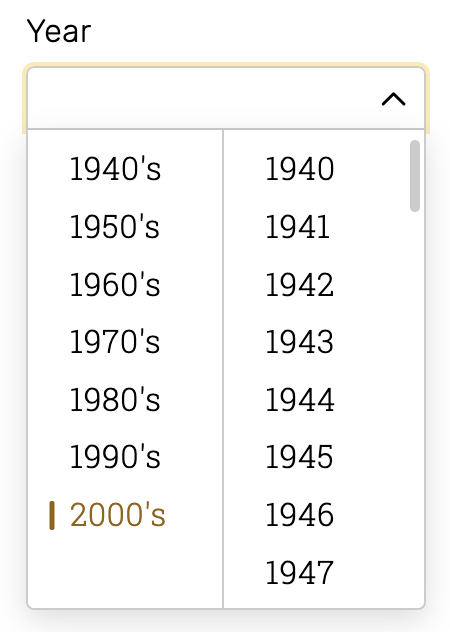
\includegraphics[width=80mm]{newComponent/opened.2col.png}
    \caption*{\centering Beispiel \codestyle{SelectComponentByCallbacks}}
    \label{api:selectComponentCbImg}
\end{figure}


% ---------
\clearpage
\subsection*{SelectComponentByTableValues}

\vspace*{6pt}
Creates an input component with the functionality: selecting an option in a given list. 

\vspace*{18pt}
\noindent
\textbf{Returns}: \codestyle{SelectComponentType}

\begin{table}[!htb] 
    \label{api:selectComponentByTableValuesReturn}
    \footnotesize
    \setlength\extrarowheight{4pt}
    \begin{tabular}{ p{3.5cm} p{3.5cm} p{6cm} }
        \toprule[1.2pt]
        \textbf{Function}     & \textbf{Type}        & \textbf{Description} \\
        \midrule
        getSelectController() & SelectControllerType &  \\
        getComponentView()    & HTMLDivElement       &  \\
        getLabelElement()     & HTMLLabelElemen      &  \\
        \bottomrule[1.2pt]
    \end{tabular}
\end{table}

\vspace*{6pt}
\noindent
\textbf{Parameters}

\begin{table}[!htb] 
    \label{api:selectComponentByTableValuesParameter}
    \footnotesize
    \setlength\extrarowheight{4pt}
    \begin{tabular}{ p{4.5cm} p{3cm} p{5.5cm} }
        \toprule[1.2pt]
        \textbf{Name}                 & \textbf{Type}    & \textbf{Description} \\
        \midrule
        selectAttributes              & SelectAttributes &  \\
        optionsTable                  & OptionsTable     &  \\
        sortColumnOptionsAlphabetical & Boolean          &  \\
        \bottomrule[1.2pt]
    \end{tabular}
\end{table}

\vspace*{6pt}
\noindent
\textbf{Example}

\begin{lstlisting}[style = htmlcssjs, label = api:selectComponentTvExample]
const selectAttribute = { name : "year", label: "Year" };
const tableOptions    = [ 
    [ "1940's", 1940 ], 
    [ "1940's", 1941 ], 
    [ "1940's", 1942 ], 
    [ "1940's", 1943 ], 
    [ "1940's", 1944 ], 
    /* ... */
    [ "1950's", 1958 ], 
    [ "1950's", 1959 ], 
    [ "1960's", 1960 ], 
    [ "1960's", 1961 ], 
    /* ... */
    [ "2000's", 2007 ], 
    [ "2000's", 2008 ], 
    [ "2000's", 2009 ], 
];

const selectComponent = SelectComponentByTableValues(
    selectAttribute,
    tableOptions
);

const componentYear   = document.getElementById("componentContainer");
componentYear.append(selectComponent.getComponentView());
\end{lstlisting}
    
\begin{figure}[!htb]
    \centering
    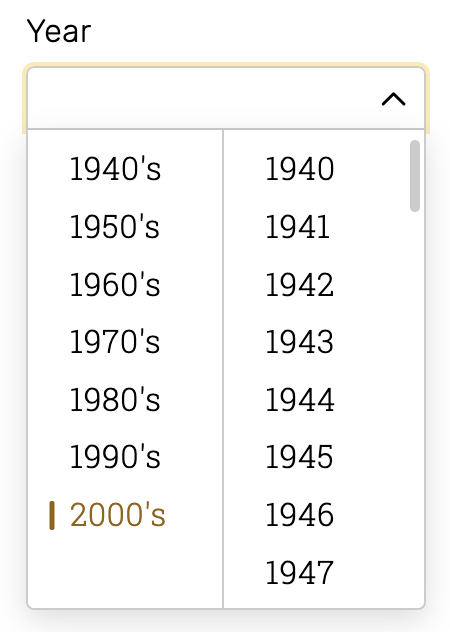
\includegraphics[width=80mm]{newComponent/opened.2col.png}
    \caption*{\centering Beispiel \codestyle{SelectComponentByTableValues}}
    \label{api:selectComponentTvImg}
\end{figure}


% ---------
\clearpage
\subsection*{ColumnOptionsComponent}

\vspace*{6pt}
Creates a column view of a given list of options. 

\vspace*{18pt}
\noindent
\textbf{Returns}: \codestyle{ColumnOptionsComponentType}

\begin{table}[!htb] 
    \label{api:columnOptionsComponentReturn}
    \footnotesize
    \setlength\extrarowheight{4pt}
    \begin{tabular}{ p{5cm} p{3cm} p{5cm} }
        \toprule[1.2pt]
        \textbf{Function}                   & \textbf{Type}     & \textbf{Description} \\
        \midrule
        getOptions()                        & Array<OptionType> &  \\
        addOptions(Array<OptionType>)       & void              &  \\
        delOptions(Array<OptionType>)       & void              &  \\
        clearOptions()                      & void              &  \\
        getSelectedOption()                 & OptionType        &  \\
        setSelectedOption(OptionType)       & void              &  \\
        clearSelectedOption()               & void              &  \\
        \tbbr{
            onOptionSelected( \\
                \ \ \ ConsumerType<OptionType>
            )}                              & void              &  \\
        isSelectedOptionDisabled()          & Boolean           &  \\
        setSelectedOptionDisabled(bool)     & void              &  \\
        \tbbr{
            onSelectedOptionDisabledChanged( \\
                \ \ \ ConsumerType<OptionType>
            )}                              & void              &  \\
        getColumnView()                     & HTMLDivElement    &  \\
        \bottomrule[1.2pt]
    \end{tabular}
\end{table}

\vspace*{6pt}
\noindent
\textbf{Parameters}

\begin{table}[!htb] 
    \label{api:columnOptionsComponentParameter}
    \footnotesize
    \setlength\extrarowheight{4pt}
    \begin{tabular}{ p{3.2cm} p{4.2cm} p{5.6cm} }
        \toprule[1.2pt]
        \textbf{Name}            & \textbf{Type}                & \textbf{Description} \\
        \midrule
        cursorPositionController & SelectedOptionControllerType &  \\
        columnNumber             & Number                       &  \\
        \bottomrule[1.2pt]
    \end{tabular}
\end{table}

\vspace*{6pt}
\noindent
\textbf{Example}

\begin{lstlisting}[style = htmlcssjs, label = api:columnOptionsComponentExample]
const cursorPos = SelectedOptionController();
const component = ColumnOptionsComponent(cursorPos);
document.getElementById("componentContainer").append(component.getColumnView());

const selectedOption = CategoryOption("selected");
const options = [ 
    selectedOption,
    CategoryOption("cat 1"),
    CategoryOption("cat 2"),
    CategoryOption("cat 3") 
];

component.addOptions(options);
component.setSelectedOption(selectedOption);

document.querySelector("head style").textContent += pageCss;
\end{lstlisting}

\begin{figure}[!htb]
    \centering
    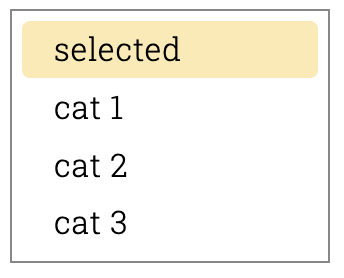
\includegraphics[width=50mm]{columnOptionsExample.png}
    \caption*{\centering Beispiel \codestyle{Column\-Options\-Component}}
    \label{api:columnOptionsComponentImg}
\end{figure}

% ---------
